\chapter{仮説}
\label{proposed}
%どうやったら解けると考えているか (検証可能なように書く)

本章では仮説について述べる。

\section{概要}
本研究では、利用規約の読解支援のために、以前同意した利用規約を記録し、それに類似する条文を読んだときに類似していることを検出し、それ以外に注目することで、利用規約の読解時間の短縮ができるのではないかと考えた。

\subsection{利用規約類似文検出}
\label{sub:利用規約類似文検出}
仮説のうち、類似条文を検出する部分について述べる。

図\ref{img:demo}では、イメージを示している。ここでは、提案するシステムを利用し始めて、初めに、A社の利用規約を読んだときは条文の背景が全て黄色で目立ち、次にB社の利用規約を読むと3がA社の1と類似する条文であるため、それ以外の条文が背景が黄色で目立ち、最後にC社の利用規約を読むと1,3,4,5が類似する条文であるため、2が背景が黄色で目立つイメージとなっている。
\begin{figure}[h]
  \begin{center}
      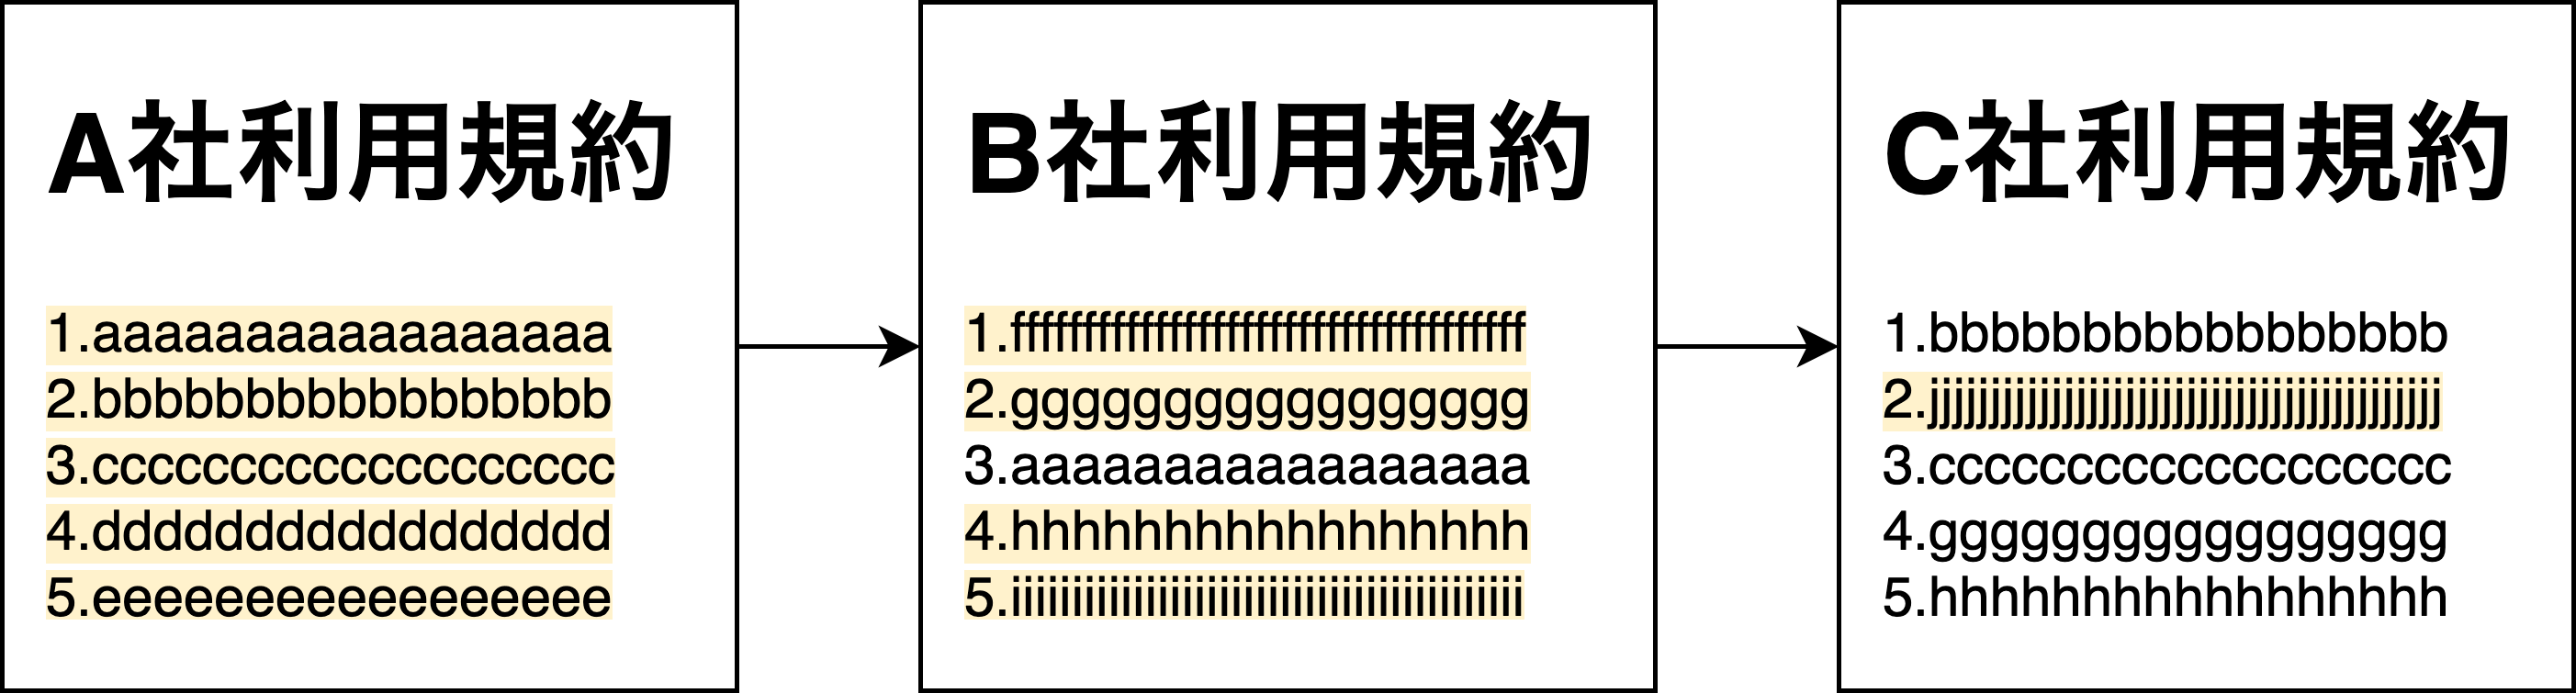
\includegraphics[width=15cm]{img/demo.drawio.png}
      \caption{類似条文検出のイメージ}
      \label{img:demo}
  \end{center}
\end{figure}

\subsection{利用規約警告検出}
\label{sub:利用規約警告検出}
\ref{sub:利用規約類似文検出}項では、利用規約の類似文を検出していったが、この仕組みの問題点として、問題があるが、サービスを利用したいために仕方なく利用したという状況が考えられる。このような状況に陥ってしまうと、提案するシステムは正しく挙動することができないため、その対策として、利用規約のうち、問題があると利用者が考えた部分について、ユーザーに指定してもらいうことで、利用規約の問題のある部分を目立たせることができる。図\ref{img:demo_warning}では、利用規約警告検出のイメージを示している。A社の1が問題ある条文であるとユーザーが考えたため、1にチェックをすると、次にB社の利用規約を読んだときにその条文と類似している3の条文の背景を水色にして目立たせる。最後に、C社の利用規約を読むと、再び類似する条文1について水色が目立つイメージとなっている。
\begin{figure}[h]
  \begin{center}
      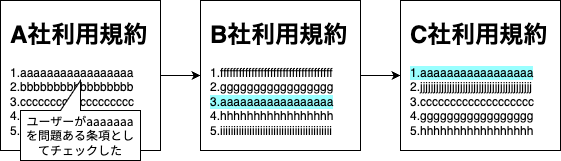
\includegraphics[width=15cm]{img/demo_warning.drawio.png}
      \caption{利用規約警告検出}
      \label{img:demo_warning}
  \end{center}
\end{figure}

%%% Local Variables:
%%% mode: japanese-latex
%%% TeX-master: "../bthesis"
%%% End:
